%%%%%%%%%%%%%%%%%%%%%%%%%%%%%%%%%%%%%%%%%%%%%%%%%%%%%%%%%%%%%%%
%
% Welcome to Overleaf --- just edit your LaTeX on the left,
% and we'll compile it for you on the right. If you open the
% 'Share' menu, you can invite other users to edit at the same
% time. See www.overleaf.com/learn for more info. Enjoy!
%
%%%%%%%%%%%%%%%%%%%%%%%%%%%%%%%%%%%%%%%%%%%%%%%%%%%%%%%%%%%%%%%
% Author: Izaak Neutelings (October 2020)
% Inspiration: https://tex.stackexchange.com/questions/25531/adding-underbrace-in-tikz
\documentclass[border=3pt,tikz]{standalone}
\usepackage{physics}
\usepackage{siunitx}
\usepackage{ifthen}
\usepackage{tikz}
%\usepackage[outline]{contour} % glow around text
\usetikzlibrary{calc}
\usetikzlibrary{angles,quotes} % for pic
\usetikzlibrary{patterns}
\tikzset{>=latex} % for LaTeX arrow head
%\contourlength{1.4pt}

\colorlet{xcol}{blue!70!black}
\colorlet{vcol}{green!70!black}
\colorlet{myred}{red!65!black}
\colorlet{acol}{red!50!blue!80!black!80}
\tikzstyle{ground}=[preaction={fill,top color=black!10,bottom color=black!5,shading angle=20},
                    fill,pattern=north east lines,draw=none,minimum width=0.3,minimum height=0.6]
\tikzstyle{metal}=[fill,top color=black!40,bottom color=black!20,shading angle=10]
\tikzstyle{mass}=[line width=0.6,red!30!black,fill=red!40!black!10,rounded corners=1,
                  top color=red!40!black!20,bottom color=red!40!black!10,shading angle=20]
\tikzstyle{rope}=[brown!70!black,very thick,line cap=round]
\def\rope#1{ \draw[black,line width=1.5] #1; \draw[rope] #1; }

% FORCES SWITCH
\tikzstyle{force}=[->,myred,very thick,line cap=round]
\tikzstyle{Fproj}=[force,myred!40]
\newcommand{\vbF}{\vb{F}}
\newcommand{\vbT}{\vb{T}}

\begin{document}


% CIRCULAR MOTION - 2D
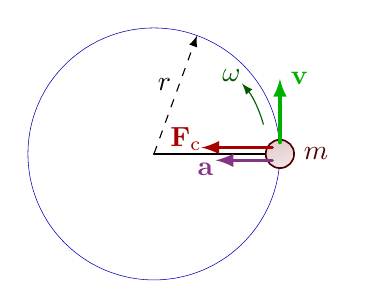
\begin{tikzpicture}
  \def\R{1.6}  % string length
  \def\r{0.18} % ball radius
  \def\Ry{0.5} % small radius of the ellipse
  \def\F{0.9}  % force size
  \coordinate (O) at (0,0);
  \coordinate (M) at (\R,0);
  \coordinate (F0) at ($(M)+(104:0.8*\r)$);
  \coordinate (F) at ($(F0)+(90:\F)$);
  \draw[very thin,xcol] (O) circle (\R);
  \draw[->,dashed] (O) -- (70:\R) node[midway,above left=-2] {$r$};
  \draw[thick,line cap=round] (O) -- (\R,0); %node[midway,above left=-2] {$r$};
  \draw[thin,mass] (M) circle (\r) node[right=5] {$m$};
  \draw[force] (M)++(140:0.7*\r) --++ (-\F,0) node[below=1,above left=-4] {$\vb{F}_\mathrm{c}$};
  \draw[force,acol] (M)++(-140:0.7*\r) --++ (-0.8*\F,0) node[below left=-3] {$\vb{a}$};
  \draw[force,vcol] (M)++(90:0.8*\r) --++ (0,0.9*\F) node[right=0] {$\vb{v}$};
  \draw[->,vcol!50!black] (15:0.9*\R) arc(15:40:0.85*\R) node[above left=-3] {$\omega$};
\end{tikzpicture}


% CIRCULAR MOTION string
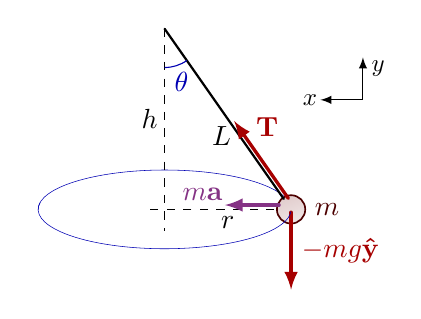
\begin{tikzpicture}
  \def\L{2.8}    % string length
  \def\r{0.18}   % ball radius
  \def\Ry{0.5}   % small radius of the ellipse
  \def\ang{35}   % angle
  \def\F{1.2}    % force size
  %\def\dang{17} % angle offset
  \coordinate (O) at (0,0);
  \coordinate (T) at (0,{\L*cos(\ang)});
  \coordinate (M) at ({\L*sin(\ang)},0);
  \coordinate (F0) at ($(M)+(104:0.8*\r)$);
  \coordinate (F) at ($(F0)+(90+\ang:\F)$);
  %\coordinate (Fy) at ($(F0)+(90:{\F*cos(\ang)})$);
  %\coordinate (Fx) at ($(F0)+(180:{\F*sin(\ang)})$);
  
  % STRING + MASS
  \draw[very thin,xcol] (M) arc (0:180:{\L*sin(\ang)} and \Ry);
  \draw[dashed] (T) -- (O) node[midway,left=-1] {$h$} -- (0,-0.1*\L);
  \draw[dashed] (M) -- (O) node[midway,below=-1] {$r$} -- (-0.1*\L,0);
  \draw[thin,mass] (M) circle (\r) node[right=5] {$m$};
  \draw[thick,line cap=round] (T) --++ (\ang-90:\L-0.9*\r) node[midway,left=1,below=1] {$L$};
  %\draw[thin,xcol] (O) ellipse ({\L*sin(\ang)} and \Ry);
  %\draw[very thin,xcol] (\dang:{\L*sin(\ang)} and \Ry) arc (\dang:358:{\L*sin(\ang)} and \Ry);
  \draw pic["$\theta$",xcol,draw=xcol,angle radius=14,angle eccentricity=1.45] {angle=O--T--M};
  
  % FORCES
  \draw[<->] (M)++(75:8*\r) node[left=-2,scale=0.9] {$x$} -|++ (3*\r,3*\r) node[below=4,right=0,scale=0.9] {$y$};
  %\draw[dashed,myred!80!black!60] (Fx) -- (F) -- (Fy);
  %\draw[force] (F0) -- (F) node[above=3,right=-1] {\contour{white}{$\vbT$}};
  \draw[force] (F0) -- (F) node[below=2,right=4] {$\vbT$};
  %\draw[Fproj] (F0) -- (Fy) node[below=2,right=0] {$\vbT_y$};
  %\draw[Fproj] (F0) -- (Fx) node[above=2,left=-3] {$\vbT_x$};
  \draw[force] (M)++(0,-0.2*\r) --++ (-90:{\F*cos(\ang)}) node[midway,right=0] {$-mg\vu{y}$};
  %\draw[force,acol] (M) --++ (180:{\F*sin(\ang)}) node[midway,below=0] {$m\vb{a}$};
  \draw[force,acol] (M)++(160:0.9*\r) --++ (180:{\F*sin(\ang)}) node[above=4,left=-3] {$m\vb{a}$};
  
  %\draw pic["$\theta$",xcol,draw=xcol,angle radius=14,angle eccentricity=1.45] {angle=Fy--F0--F};
  %\draw pic["$\theta_3$",xcol,draw=xcol,angle radius=13,angle eccentricity=1.40] {angle=F3--O--T};
  \draw[very thin,xcol] (170:{\L*sin(\ang)} and \Ry) arc (170:357:{\L*sin(\ang)} and \Ry);
\end{tikzpicture}


% CIRCULAR MOTION - force balance
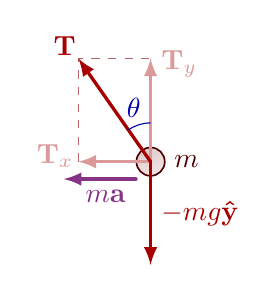
\begin{tikzpicture}
  \def\ang{35}   % angle
  \def\F{1.6}    % force size
  \def\r{0.18}   % ball radius
  \coordinate (O) at (0,0);
  \coordinate (F) at (90+\ang:\F);
  \coordinate (Fy) at (90:{\F*cos(\ang)});
  \coordinate (Fx) at (180:{\F*sin(\ang)});
  \draw[thin,mass] (O) circle (\r) node[right=5] {$m$};
  \draw[dashed,myred!80!black!60] (Fx) -- (F) -- (Fy);
  \draw[Fproj] (O) -- (Fy) node[below=2,right=0] {$\vbT_y$};
  \draw[Fproj] (O) -- (Fx) node[above=2,left=-2] {$\vbT_x$};
  \draw[force] (O) -- (F) node[above left=-3] {$\vbT$};
  \draw[force] (O) --++ (-90:{\F*cos(\ang)}) node[midway,right=0] {$-mg\vu{y}$};
  \draw[force,acol] (O)++(-130:1.6*\r) --++ (Fx) node[midway,right=2,below=0] {$m\vb{a}$};
  \draw pic["$\theta$",xcol,draw=xcol,angle radius=14,angle eccentricity=1.45] {angle=Fy--O--F};
\end{tikzpicture}


% CIRCULAR MOTION - force balance - tip to toe (or but?)
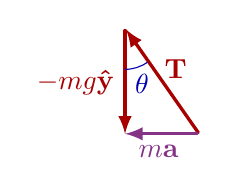
\begin{tikzpicture}
  \def\ang{35}   % angle
  \def\F{1.6}    % force size
  \def\r{0.18}   % ball radius
  \coordinate (O) at (0,0);
  \coordinate (F) at ((90+\ang:\F);
  \coordinate (Fx) at (180:{\F*sin(\ang)});
  \draw[force] (90-\ang:0.02) --++ (F) node[midway,above right=-3] {$\vbT$};
  \draw[force] (F) -- (Fx) node[midway,left=0] {$-mg\vu{y}$};
  \draw[force,acol] (O) -- (Fx) node[midway,left=1,below=0] {$m\vb{a}$};
  \draw pic["$\theta$",xcol,draw=xcol,angle radius=14,angle eccentricity=1.45] {angle=Fx--F--O};
\end{tikzpicture}


\end{document}